%-------------------------------------------------------------------------------
% 请勿删除本注释
% Free Response Question 3
%
% 指引:
% 如在小问之前有通用问题描述,请放置于此
%-------------------------------------------------------------------------------
\begin{figure}[H]
\centering
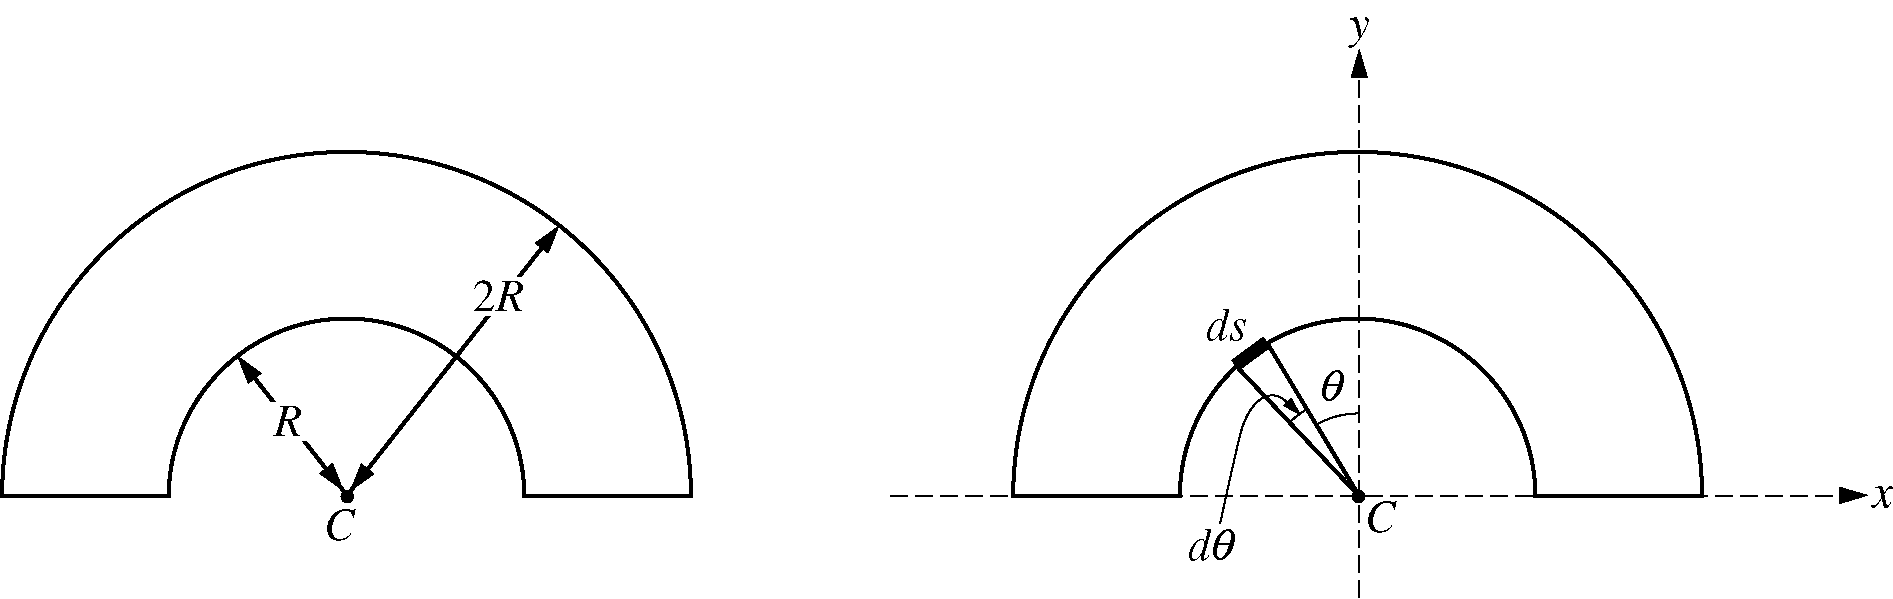
\includegraphics[scale=0.2]{images/img-020-045.png}
\end{figure}


\question
A thin nonconducting wire is shaped into a loop containing two concentric semicircular arcs with their centers at point $C$, as shown above. The wire carries a positive uniform linear charge density $\lambda$. Express your answers in parts (a) and (b) in terms of $R, \lambda, \theta$, and fundamental constants, as appropriate. % 请删除并替换本行,与上一行 \question 之间不要留空行

\begin{parts}

%-------------------------------------------------------------------------------
% 请勿删除本注释
% Part (a)
%
% 指引:
% 如在小问之前有通用问题描述,请放置于此
%-------------------------------------------------------------------------------

\part
Derive an expression for the $y$-component of the infinitesimally small electric field, $d E_{y}$, produced at point $C$ by the charge on the small piece of wire in terms of the infinitesimally small angle $d \theta$ shown in the figure on the right. % 请删除并替换本行,与上一行 \part 之间不要留空行

%-------------------------------------------------------------------------------
% 请勿删除本注释
% Part (b)
%
% 指引:
% 如在小问之前有通用问题描述,请放置于此
%-------------------------------------------------------------------------------

\part
Using the expression from part (a), derive an expression for the magnitude of the electric field at point $C$ produced by the entire wire. % 请删除并替换本行,与上一行 \part 之间不要留空行

%-------------------------------------------------------------------------------
% 请勿删除本注释
% Part (c)
%
% 指引:
% 如在小问之前有通用问题描述,请放置于此
%-------------------------------------------------------------------------------

The nonconducting wire is replaced by an uncharged conducting wire with the same size and shape, which has some electrical resistance. A battery is inserted into the loop, as shown below, resulting in a current $I$ in the wire.


\begin{figure}[H]
\centering
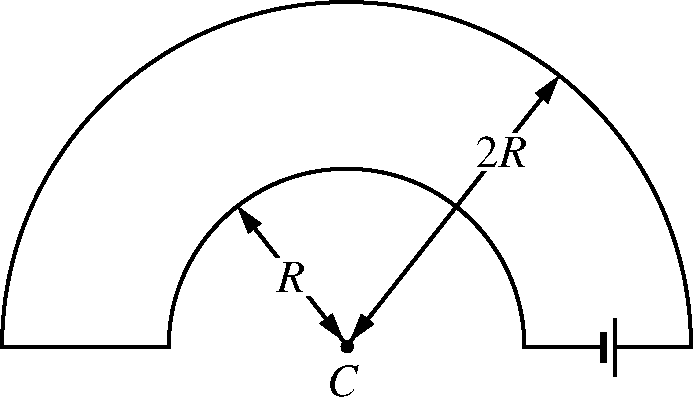
\includegraphics[scale=0.3]{images/img-021-046.png}
\end{figure}

\part
Determine the direction of the magnetic field at point  $C$. Explain your reasoning.  % 请删除并替换本行,与上一行 \part 之间不要留空行

%-------------------------------------------------------------------------------
% 请勿删除本注释
% Part (d)
%
% 指引:
% 如在小问之前有通用问题描述,请放置于此
%-------------------------------------------------------------------------------

\part
Using the Biot-Savart law, derive an expression for the magnitude of the magnetic field $B$ at point $C$. Express your answers in terms of $R, I$, and fundamental constants, as appropriate. % 请删除并替换本行,与上一行 \part 之间不要留空行

\end{parts}
